\documentclass[12pt,a4paper]{article}
\title{Linear Regression}
\author{Hanxiao Du}
\date{}

\usepackage{amsmath}
\usepackage{amssymb}
\usepackage{amsthm}
\usepackage{bbm}
\usepackage{pifont}
\usepackage{marvosym}
\usepackage{mathtools}
\usepackage{environ}
\usepackage{lipsum}
\usepackage{undertilde}
\usepackage{hyperref}
\usepackage{graphicx}
\hypersetup{colorlinks=true,
     linkcolor=black,urlcolor=blue}

\usepackage[total={6in, 10in}]{geometry}
\newtheorem{theorem}{Theorem}
\setlength{\parindent}{0pt}
\renewcommand{\qedsymbol}{$\blacksquare$}
\DeclareMathOperator*{\argmax}{\arg\!\max}
\DeclareMathOperator*{\argmin}{\arg\!\min}

\begin{document}
\maketitle
\tableofcontents

\section{Introduction}

Although linear regression can be used in classification tasks, it
usually performs poorly. For example, instances that are far from the
centroid could drag the regression line so that the linear regression
cannot yield a proper dicision boundary (see figure \ref{linear_reg}).

\begin{figure}[h]
\centering
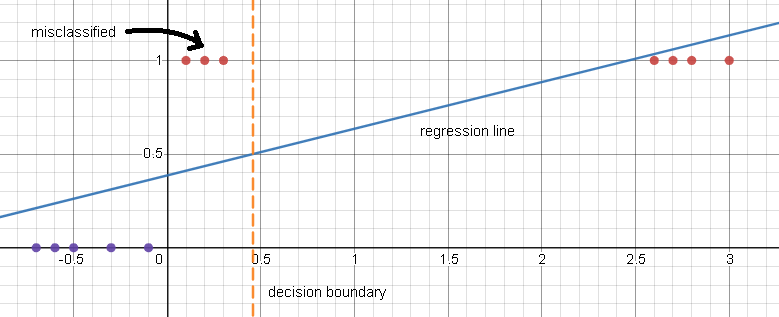
\includegraphics[scale=0.7]{assets/figures/linear_reg.png}
\caption{Linear regression as a classifier.\label{linear_reg}}
\end{figure}

Logistic regression can solve this issue by fitting the data with
logistic (sigmoid) function (see figure \ref{sigmoid}):

\begin{align}\label{sigmoid_func}
\sigma(z)=\frac{1}{1+e^{-z}} = \frac{e^z}{e^{z}+1} = 1-\sigma(-z)
\end{align}

\begin{figure}[h]
\centering
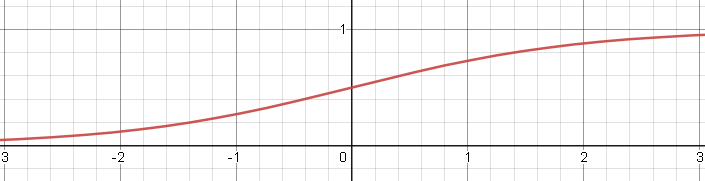
\includegraphics[scale=0.7]{assets/figures/sigmoid.png}
\caption{Logistic (sigmoid) function.\label{sigmoid}}
\end{figure}

\section{Hypothesis}

Logistic regression assumes the real binary outcome random variable
${Y = \mathbb{I}(X\beta + \epsilon \geq 0)}$, where
\(\mathbb{I}(\cdot)\) is the indicator function, $X$ is the
independent random variable, \(\beta\) is the parameter (coefficent)
vector and $\epsilon$ is the error term matrix. The distribution of
the error term $\epsilon$ conditional on $X=x$ is
$\epsilon | X=x \sim Logistic(\mu=0, s=1)$.

The logistic distribution $Logistic(\mu=0, s=1)$ has the sigmoid
function as its cumulative distribution function(CDF):
\begin{align}\label{logistic_CDF}
F(z)=\sigma(z)=\frac{1}{1+e^{-z}}
\end{align}

Thus, the probability of the outcome variable $Y=1$ given $X$ can be
calculated as: \begin{align}
\mathbb{P}(Y=1|X=x) &= \mathbb{P}(X\beta + \epsilon \geq 0|X=x)\\
&=\mathbb{P}(\epsilon \geq -X\beta|X=x)\\
&=1-\mathbb{P}(\epsilon < -X\beta|X=x)\\
&=1-F(-x^T\beta)\text{, where } F \text{ is the CDF defined in (\ref{logistic_CDF})}\\
&=1-\sigma(-x^T\beta)\\
&=1-(1-\sigma(x^T\beta))\text{, by (\ref{sigmoid_func})}\\
&=\frac{1}{1+e^{-x^T\beta}}
\end{align}

Then, we can model $\mathbb{P}(Y=1|X=x)$ by $h_\beta(x)=\sigma(x^T\beta)=\frac{1}{1+e^{-x^T\beta}}$

Additionally,
\begin{align}
\mathbb{P}(Y=1|X=x) = \frac{1}{1+e^{-x^T\beta}}&\iff \frac{1-\mathbb{P}(Y=1|X=x)}{\mathbb{P}(Y=1|X=x)} = e^{-x^T\beta}\\
&\iff \frac{\mathbb{P}(Y=1|X=x)}{1-\mathbb{P}(Y=1|X-x)} = e^{x^T\beta}\\
&\iff log(\frac{\mathbb{P}(Y=1|X=x)}{1-\mathbb{P}(Y=1|X=x)}) = x^T\beta\\
&\iff logit(\mathbb{P}(Y=1|X=x)) = x^T\beta
\end{align}
where
\begin{align}
logit(p) = log(\frac{p}{1-p}) = \sigma^{-1}(p)
\end{align}

\section{Decision Boundary}
The decision boundary of logistic regression is $\mathbb{P}(Y=1|X=x) = 0.5$, since when ${\mathbb{P}(Y=1|X=x) > 0.5}$, the model suggests that $\mathbb{P}(Y=1|X=x) > \mathbb{P}(Y=0|X=x)$ and vice versa.\\

Or equivalently,
\begin{align}
\mathbb{P}(Y=1|X=x)= \frac{1}{1+e^{-x^T\beta}} = 0.5 \iff x^T\beta = 0
\end{align}

\section{Cost Function}
The loss function for logistic regression is normally the binary cross entropy, thus we have the cost:
\begin{align}
J(\beta)&=H_\beta(\utilde{y}, \utilde{\hat{y}})=-||\utilde{y}log(h_\beta(\utilde{x}))+(\utilde{1}-\utilde{y})log(1-h_\beta(\utilde{x}))||^2\\
&=-\sum_{i=1}^n \Big[y_ilog(h_\beta(x_i)) + (1-y_i)log(1-h_\beta(x_i))\Big]\\
&=-\sum_{i=1}^n \Big[y_ilog(\frac{1}{1+e^{-x_i^T\beta}}) + (1-y_i)log(1-\frac{1}{1+e^{-x_i^T\beta}})\Big]\\
&=-\sum_{i=1}^n \Big[y_ilog(\frac{1}{1+e^{-x_i^T\beta}}) + (1-y_i)log(\frac{e^{-x_i^T\beta}}{1+e^{-x_i^T\beta}})\Big]
\end{align}

The reason why we do not use the mean squared error as the cost function is that we cannot guarantee the convexity of the mean squared error when it is applied to logistic regression.

\begin{theorem}
$J(\beta)$ is convex.
\begin{proof}
\begin{align}
\frac{\partial J(\beta)}{\partial \beta}&=-\sum_{i=1}^n \Big[y_i\frac{e^{-x_i^T\beta}}{1+e^{-x_i^T\beta}}x_i - (1-y_i)\frac{1}{1+e^{-x_i^T\beta}}x_i\Big]\\
&=-\sum_{i=1}^n \Big[y_i(1-h_\beta(x_i))x_i- (1-y_i)h_\beta(x_i)x_i\Big]\\
&=-\sum_{i=1}^n \Big[y_i-y_i h_\beta(x_i)- h_\beta(x_i)+y_ih_\beta(x_i)\Big]x_i\\
&=-\sum_{i=1}^n \Big[y_i- h_\beta(x_i)\Big]x_i\\
&=-\sum_{i=1}^n \Big[y_i- \sigma(x_i^T\beta)\Big]x_i\\
&=\sum_{i=1}^n \Big[\sigma(x_i^T\beta)-y_i\Big]x_i\\
&=\sum_{i=1}^n \Big[\frac{1}{1+e^{-x_i^T\beta}}-y_i\Big]x_i
\end{align}

\begin{align}
\frac{\partial^2 J(\beta)}{\partial \beta^2}=\frac{\partial}{\partial \beta} \Big(\frac{\partial J(\beta)}{\partial \beta}\Big) &=\sum_{i=1}^n  \frac{e^{-x_i^T\beta}}{(1+e^{-x_i^T\beta})^2}x_ix_i^T
\end{align}
where $x_ix_i^T$ is always positive semi-definite.

Thus, $\frac{\partial^2 J(\beta)}{\partial \beta^2}$ is always positive semi-definite, which implies that $J(\beta)$ is convex.\\
\end{proof}
\end{theorem}

There is no analytical solution for $\hat{\beta}=\underset{\beta}\argmin J(\beta)$. Gradient descent technique can be used to find the numerical approximation of $\hat{\beta}$:

\begin{align}
\beta_{t+1} \leftarrow \beta_{t} - \eta \frac{\partial J(\beta)}{\partial \beta} = \beta_{t} -\eta \sum_{i=1}^n \Big[\sigma(x_i^T\beta)-y_i\Big]x_i
\end{align}
\end{document}

